\documentclass[a4paper, justified]{tufte-handout}\usepackage[]{graphicx}\usepackage[]{xcolor}
% maxwidth is the original width if it is less than linewidth
% otherwise use linewidth (to make sure the graphics do not exceed the margin)
\makeatletter
\def\maxwidth{ %
  \ifdim\Gin@nat@width>\linewidth
    \linewidth
  \else
    \Gin@nat@width
  \fi
}
\makeatother

\definecolor{fgcolor}{rgb}{0.345, 0.345, 0.345}
\newcommand{\hlnum}[1]{\textcolor[rgb]{0.686,0.059,0.569}{#1}}%
\newcommand{\hlstr}[1]{\textcolor[rgb]{0.192,0.494,0.8}{#1}}%
\newcommand{\hlcom}[1]{\textcolor[rgb]{0.678,0.584,0.686}{\textit{#1}}}%
\newcommand{\hlopt}[1]{\textcolor[rgb]{0,0,0}{#1}}%
\newcommand{\hlstd}[1]{\textcolor[rgb]{0.345,0.345,0.345}{#1}}%
\newcommand{\hlkwa}[1]{\textcolor[rgb]{0.161,0.373,0.58}{\textbf{#1}}}%
\newcommand{\hlkwb}[1]{\textcolor[rgb]{0.69,0.353,0.396}{#1}}%
\newcommand{\hlkwc}[1]{\textcolor[rgb]{0.333,0.667,0.333}{#1}}%
\newcommand{\hlkwd}[1]{\textcolor[rgb]{0.737,0.353,0.396}{\textbf{#1}}}%
\let\hlipl\hlkwb

\usepackage{framed}
\makeatletter
\newenvironment{kframe}{%
 \def\at@end@of@kframe{}%
 \ifinner\ifhmode%
  \def\at@end@of@kframe{\end{minipage}}%
  \begin{minipage}{\columnwidth}%
 \fi\fi%
 \def\FrameCommand##1{\hskip\@totalleftmargin \hskip-\fboxsep
 \colorbox{shadecolor}{##1}\hskip-\fboxsep
     % There is no \\@totalrightmargin, so:
     \hskip-\linewidth \hskip-\@totalleftmargin \hskip\columnwidth}%
 \MakeFramed {\advance\hsize-\width
   \@totalleftmargin\z@ \linewidth\hsize
   \@setminipage}}%
 {\par\unskip\endMakeFramed%
 \at@end@of@kframe}
\makeatother

\definecolor{shadecolor}{rgb}{.97, .97, .97}
\definecolor{messagecolor}{rgb}{0, 0, 0}
\definecolor{warningcolor}{rgb}{1, 0, 1}
\definecolor{errorcolor}{rgb}{1, 0, 0}
\newenvironment{knitrout}{}{} % an empty environment to be redefined in TeX

\usepackage{alltt}
\geometry{
  left=24.8mm, % left margin
  textwidth=100mm, % main text block
  marginparsep=3mm, % gutter between main text block and margin notes
  marginparwidth=75mm % width of margin notes
}
% Packages {
  \usepackage[portuguese]{babel}
  % KableExtra {
    \usepackage{booktabs}
    \usepackage{longtable}
    \usepackage{array}
    \usepackage{multirow}
    \usepackage{wrapfig}
    \usepackage{float}
    \usepackage{colortbl}
    \usepackage{pdflscape}
    \usepackage{tabu}
    \usepackage{threeparttable}
    \usepackage{threeparttablex}
    \usepackage[normalem]{ulem}
    \usepackage{makecell}
    \usepackage{xcolor}
  % }
% }



% Titulo {
  \title{TODO TITULO}
  \author{
    André Planhca, 105289 \\
    <Andre\_Plancha@iscte-iul.pt> \\
    Tomás Ribeiro, 105220 \\
    <tfroo1@iscte-iul.pt> \\
    TODO AUTOR, NUMERO \\
    <TODO EMAIL> \\
    TODO AUTOR, NUMERO \\
    <TODO EMAIL>
  }
  \date{20/11/2022 \\ Versão 0.0.1} % 
% }

% { bug workaround (https://github.com/Tufte-LaTeX/tufte-latex/issues/64#issuecomment-78572017)
\renewcommand\allcapsspacing[1]{{\addfontfeature{LetterSpace=15}#1}}
\renewcommand\smallcapsspacing[1]{{\addfontfeature{LetterSpace=10}#1}}
% }
% {R code and table
\newenvironment{RTable}[1]{\begin{margintable}\begin{center}\begin{tabular}{#1}}{\end{tabular}\end{center}\end{margintable}}
% }

\bibliography{references.bib}
\IfFileExists{upquote.sty}{\usepackage{upquote}}{}
\begin{document}


% cover { 
  \cleardoublepage
  {
  \sffamily
  \begin{fullwidth}
  \fontsize{18}{20}\selectfont\par\noindent\textcolor{darkgray}{\allcaps{\thanklessauthor}}%
  \vspace{11.5pc}
  \fontsize{36}{40}\selectfont\par\noindent\textcolor{darkgray}{\allcaps{\thanklesstitle}}%
  \vfill
  \fontsize{14}{16}\selectfont\par\noindent\allcaps{\thanklesspublisher}
  \end{fullwidth}
  }
  \thispagestyle{empty}
  \clearpage
% }

Hello world

\begin{knitrout}
\definecolor{shadecolor}{rgb}{0.969, 0.969, 0.969}\color{fgcolor}\begin{kframe}
\begin{alltt}
\hlstd{listings} \hlkwb{<-} \hlkwd{read.csv}\hlstd{(}\hlkwd{here}\hlstd{(}\hlstr{"listings.csv"}\hlstd{))}
\hlkwd{data.frame}\hlstd{(}
  \hlkwc{row.names} \hlstd{=} \hlkwd{colnames}\hlstd{(listings),}
  \hlstr{"type"} \hlstd{=} \hlkwd{sapply}\hlstd{(listings, class)}
\hlstd{)} \hlopt \hlkwd{showT}\hlstd{()}
\end{alltt}
\end{kframe}\begingroup\fontsize{10}{12}\selectfont

\begin{RTable}{l|l}
\hline
  & type\\
\hline
\cellcolor{gray!6}{id} & \cellcolor{gray!6}{numeric}\\
\hline
name & character\\
\hline
\cellcolor{gray!6}{host\_id} & \cellcolor{gray!6}{integer}\\
\hline
host\_name & character\\
\hline
\cellcolor{gray!6}{neighbourhood\_group} & \cellcolor{gray!6}{logical}\\
\hline
neighbourhood & character\\
\hline
\cellcolor{gray!6}{latitude} & \cellcolor{gray!6}{numeric}\\
\hline
longitude & numeric\\
\hline
\cellcolor{gray!6}{room\_type} & \cellcolor{gray!6}{character}\\
\hline
price & integer\\
\hline
\cellcolor{gray!6}{minimum\_nights} & \cellcolor{gray!6}{integer}\\
\hline
number\_of\_reviews & integer\\
\hline
\cellcolor{gray!6}{last\_review} & \cellcolor{gray!6}{character}\\
\hline
reviews\_per\_month & numeric\\
\hline
\cellcolor{gray!6}{calculated\_host\_listings\_count} & \cellcolor{gray!6}{integer}\\
\hline
availability\_365 & integer\\
\hline
\cellcolor{gray!6}{number\_of\_reviews\_ltm} & \cellcolor{gray!6}{integer}\\
\hline
license & character\\
\hline
\end{RTable}
\endgroup{}

\end{knitrout}

\begin{knitrout}
\definecolor{shadecolor}{rgb}{0.969, 0.969, 0.969}\color{fgcolor}\begin{kframe}
\begin{alltt}
\hlkwd{ggplot}\hlstd{(listings,} \hlkwd{aes}\hlstd{(}\hlkwc{x}\hlstd{= price ))} \hlopt{+}
  \hlkwd{geom_density}\hlstd{()} \hlopt{+}
  \hlkwd{coord_cartesian}\hlstd{(}\hlkwc{xlim} \hlstd{=} \hlkwd{c}\hlstd{(}\hlnum{0}\hlstd{,} \hlnum{1000}\hlstd{))}
\end{alltt}
\end{kframe}\begin{marginfigure}
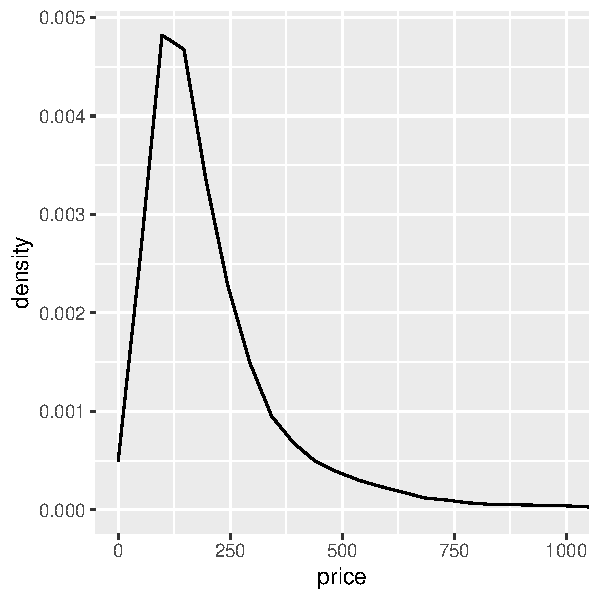
\includegraphics[width=\maxwidth]{figure/graphTest-1} \caption[ ]{ }\label{fig:graphTest}
\end{marginfigure}

\end{knitrout}

\end{document}
